\section{Análise de desempenho}

%-----------------------------------------------------------------------------
\begin{frame}[fragile]{Desempenho para processamento em tempo real}
Perguntas:
\begin{itemize}
  \item Qual é número máximo de operações computáveis em tempo real?
  \item Quais detalhes de implementação fazem diferença?
  \item Qual é a qualidade do áudio resultante?
\end{itemize}
\vspace{2em}
Implementações:
\begin{itemize}
  \item Síntese aditiva.
  \item Convolução no domínio do tempo.
  \item FFT.
\end{itemize}
\end{frame}
%-----------------------------------------------------------------------------

%-----------------------------------------------------------------------------
%     _       _     _ _ _   _             ____              _   _     
%    / \   __| | __| (_) |_(_)_   _____  / ___| _   _ _ __ | |_| |__  
%   / _ \ / _` |/ _` | | __| \ \ / / _ \ \___ \| | | | '_ \| __| '_ \ 
%  / ___ \ (_| | (_| | | |_| |\ V /  __/  ___) | |_| | | | | |_| | | |
% /_/   \_\__,_|\__,_|_|\__|_| \_/ \___| |____/ \__, |_| |_|\__|_| |_|
%                                               |___/
%-----------------------------------------------------------------------------

\subsection{Síntese Aditiva}

%-----------------------------------------------------------------------------
\begin{frame}{Síntese aditiva}
\begin{figure}
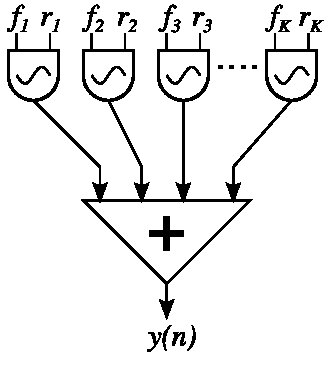
\includegraphics[height=0.8\textheight]{./img/add.pdf}
\end{figure}
\end{frame}
%-----------------------------------------------------------------------------

%-----------------------------------------------------------------------------
\begin{frame}[fragile]{Síntese aditiva}
\noindent Código em alto nível:
\begin{lstlisting}
for (n = 0; n < N; n++)
{
  angle = 2.0 * M_PI * t;
  y[n] = 0.0;
  for (k = 0; k < numFreqs; k++)
    y[n] += r[k]*sin(f[k] * angle);
  t += 1.0 / SR;
}
\end{lstlisting}
Implementação da linha 6:
\begin{lstlisting}
  ind[k] = (ind[k]+f[k]) & (SINETABLE_SIZE-1);
  y[n&(BUFFER_SIZE-1)] += sine[ind[k]] >> pad;
\end{lstlisting}
\end{frame}
%-----------------------------------------------------------------------------


%-----------------------------------------------------------------------------
\begin{frame}{Síntese aditiva}{Tipo e número de operações fazem a diferença}
%\begin{itemize}
%  \item Taxa de amostragem: $R = 31.250$~Hz (freq. até 15.625~Hz).
%  \item Tamanhos de bloco: 128 amostras.
%  \item Período do ciclo DSP: $T=\frac{N}{R}=4,096$~ms.
%\end{itemize}
\begin{figure}
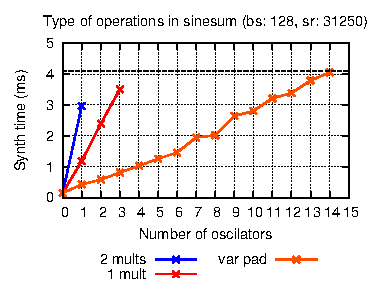
\includegraphics[width=0.8\textwidth]{./img/operations-128-31250.pdf}
\end{figure}
\end{frame}
%-----------------------------------------------------------------------------

%-----------------------------------------------------------------------------
\begin{frame}{Síntese aditiva}{Resultados para blocos de diferentes tamanhos}
%\begin{itemize}
%  \item Taxa de amostragem: $R = 31.250$~Hz (freq. até 15.625~Hz).
%  \item Tamanhos de bloco: 32, 64 e 128 amostras.
%  \item Período do ciclo DSP: $T=\frac{N}{R}$.
%\end{itemize}
\begin{figure}
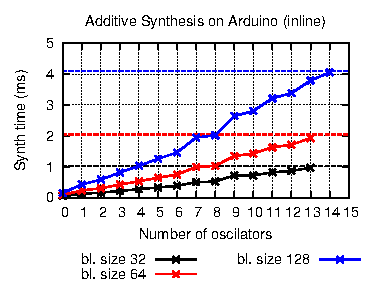
\includegraphics[width=0.8\textwidth]{./img/sinesum-comparison.pdf}
\end{figure}
\end{frame}
%-----------------------------------------------------------------------------

%-----------------------------------------------------------------------------
\begin{frame}{Síntese aditiva}{Resultados para blocos de diferentes tamanhos}
%\begin{itemize}
%  \item Taxa de amostragem: $R = 31.250$~Hz (freq. até 15.625~Hz).
%  \item Tamanhos de bloco: 32, 64 e 128 amostras.
%  \item Período do ciclo DSP: $T=\frac{N}{R}$.
%\end{itemize}
\begin{figure}
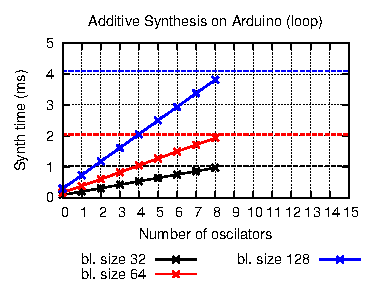
\includegraphics[width=0.8\textwidth]{./img/sinesum-comparison-for.pdf}
\end{figure}
\end{frame}
%-----------------------------------------------------------------------------


%-----------------------------------------------------------------------------
\begin{frame}{Síntese aditiva}{Resultados para diferentes taxas de amostragem}
%\begin{itemize}
%  \item Taxas de amostragem: $R_1 = 31.250$~Hz e $R_2=15.625$~Hz.
%  \item Tamanhos de bloco: 128 amostras.
%  \item Período do ciclo DSP: $T=\frac{N}{R}=8,192$~ms.
%\end{itemize}
\begin{figure}
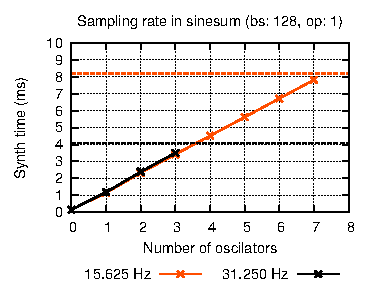
\includegraphics[width=0.8\textwidth]{./img/frequencies-128-1.pdf}
\end{figure}
\end{frame}
%-----------------------------------------------------------------------------

%-----------------------------------------------------------------------------
\begin{frame}{Síntese aditiva}{Resumo dos resultados}
Número de osciladores máximo em cada cenário ($R=31.250$~Hz):
\begin{center}
\begin{tabular}{rcccc}
\toprule
\toprule
block size  & 2op & 1op & pad+for & pad \\
\midrule
32  & 2 & 4 & 8 & 14 \\
64  & 2 & 4 & 8 & 14 \\
128 & 2 & 4 & 8 & 15 \\
\bottomrule
\end{tabular}
\pause
\end{center}
\begin{itemize}
  \item Exemplo: soma de harmônicos de 200~Hz.
\end{itemize}
\end{frame}
%-----------------------------------------------------------------------------


%-----------------------------------------------------------------------------
%   ____                      _       _   _             
%  / ___|___  _ ____   _____ | |_   _| |_(_) ___  _ __  
% | |   / _ \| '_ \ \ / / _ \| | | | | __| |/ _ \| '_ \ 
% | |__| (_) | | | \ V / (_) | | |_| | |_| | (_) | | | |
%  \____\___/|_| |_|\_/ \___/|_|\__,_|\__|_|\___/|_| |_|
%                                                       
%-----------------------------------------------------------------------------

\subsection{Convolução no domínio do tempo}

%-----------------------------------------------------------------------------
\begin{frame}{Convolução no domínio do tempo}
\begin{figure}
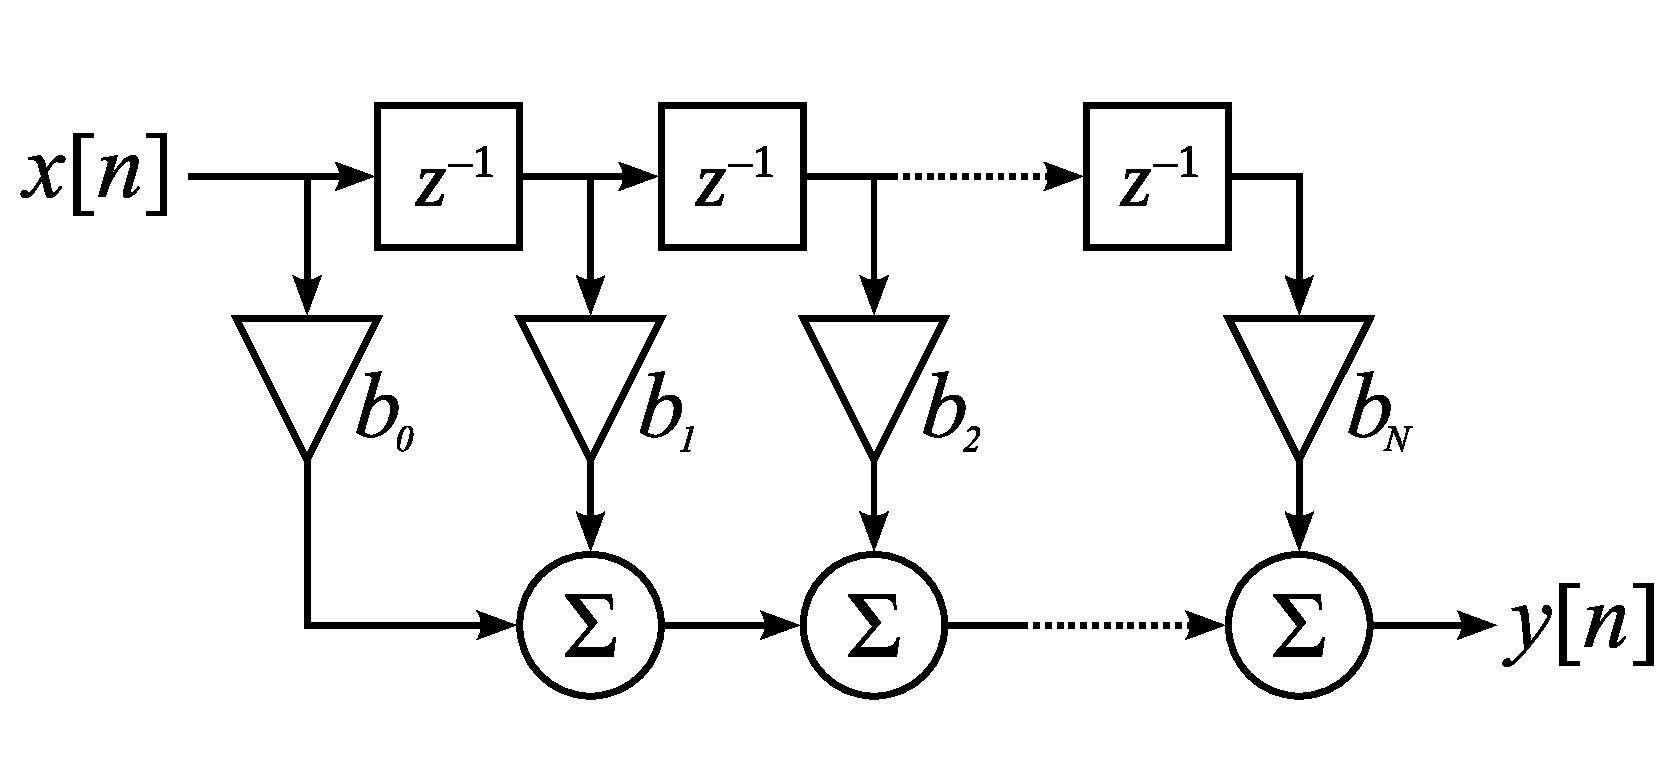
\includegraphics[width=\textwidth]{./img/FIR_Filter.pdf}
\end{figure}
\end{frame}
%-----------------------------------------------------------------------------

%-----------------------------------------------------------------------------
\begin{frame}[fragile]{Convolução no domínio do tempo}
{Qual o tamanho máximo de um filtro computável em tempo real?}
Código em alto nível:
\begin{lstlisting}
for (k = 0; k < N; k++)
  y[n] += b[k]*x[n-k];
\end{lstlisting}
Implementação:
\begin{lstlisting}
for (int n = 0; n < N; n++) {
  int yn = 0, xtmp;
  for (int i = 0; i < order; i++) {
    xtmp = 127 - TMOD(x, n-i, BUFFER_SIZE);
    yn += xtmp * 10 / 100;
  }
  LIMIT(yn); /* limita a +- 127 */
  TMOD(y, n, BUFFER_SIZE) = 127 + yn;
}
\end{lstlisting}
\end{frame}
%-----------------------------------------------------------------------------

%-----------------------------------------------------------------------------
\begin{frame}{Convolução no domínio do tempo}{Resultados para blocos de diferentes tamanhos}
%\begin{itemize}
%  \item Taxa de amostragem: $R = 31.250~Hz$.
%  \item Tamanhos de bloco: 32, 64, 128 e 256 amostras.
%  \item Tipo de operação: pad constante.
%\end{itemize}
\begin{figure}
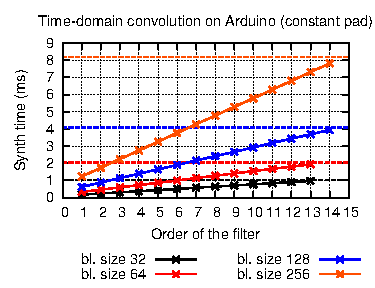
\includegraphics[width=0.8\textwidth]{./img/convolution-comparison-cpad.pdf}
\end{figure}
\end{frame}
%-----------------------------------------------------------------------------


%-----------------------------------------------------------------------------
\begin{frame}{Convolução no domínio do tempo}{Resultados para blocos de diferentes tamanhos}
%\begin{itemize}
%  \item Taxa de amostragem: $R = 31.250~Hz$.
%  \item Tamanhos de bloco: 32, 64, 128 e 256 amostras.
%  \item Tipo de operação: pad variável.
%\end{itemize}
\begin{figure}
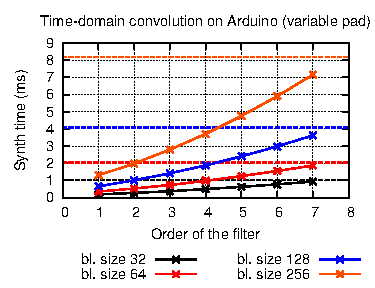
\includegraphics[width=0.8\textwidth]{./img/convolution-comparison-vpad.pdf}
\end{figure}
\end{frame}
%-----------------------------------------------------------------------------


%-----------------------------------------------------------------------------
\begin{frame}{Convolução no domínio do tempo}{Resultados para blocos de diferentes tamanhos}
%\begin{itemize}
%  \item Taxa de amostragem: $R = 31.250~Hz$.
%  \item Tamanhos de bloco: 32, 64, 128 e 256 amostras.
%  \item Tipo de operação: multiplicação.
%\end{itemize}
\begin{figure}
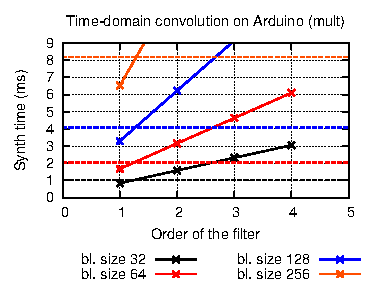
\includegraphics[width=0.8\textwidth]{./img/convolution-comparison-mult.pdf}
\end{figure}
\end{frame}
%-----------------------------------------------------------------------------

%-----------------------------------------------------------------------------
\begin{frame}{Convolução no domínio do tempo}{Resultados para blocos de diferentes tamanhos}
Ordem máxima do filtro FIR em cada cenário ($R=31.250$~Hz):
\begin{center}
\begin{tabular}{rccc}
\toprule
\toprule
\footnotesize{block size}  & \footnotesize{multiplicação} & \footnotesize{pad variável} & \footnotesize{pad constante} \\
\midrule
32  & 1 & 7 & 13 \\
64  & 1 & 7 & 13 \\
128 & 1 & 7 & 14 \\
256 & 1 & 7 & 14 \\
\bottomrule
\end{tabular}
\end{center}
\end{frame}
%-----------------------------------------------------------------------------

%-----------------------------------------------------------------------------
\begin{frame}{Convolução no domínio do tempo}{Exemplo: moving average}
%\begin{itemize}
%  \item Taxa de amostragem: $R = 31.250~Hz$.
%  \item Tamanhos de bloco: 32, 64, 128 e 256 amostras.
%  \item Tipo de operação: pad variável.
%\end{itemize}
\begin{figure}
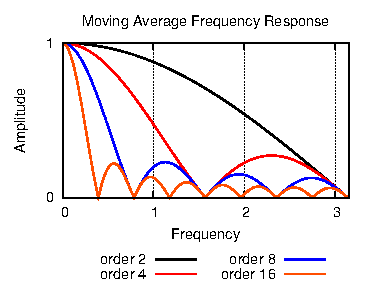
\includegraphics[width=0.8\textwidth]{./img/moving.pdf}
\end{figure}
\end{frame}
%-----------------------------------------------------------------------------

%-----------------------------------------------------------------------------
%  _____ _____ _____ 
% |  ___|  ___|_   _|
% | |_  | |_    | |  
% |  _| |  _|   | |  
% |_|   |_|     |_|  
%
%-----------------------------------------------------------------------------
\subsection{FFT}

%-----------------------------------------------------------------------------
\begin{frame}{Fast Fourier Transform}
\begin{figure}
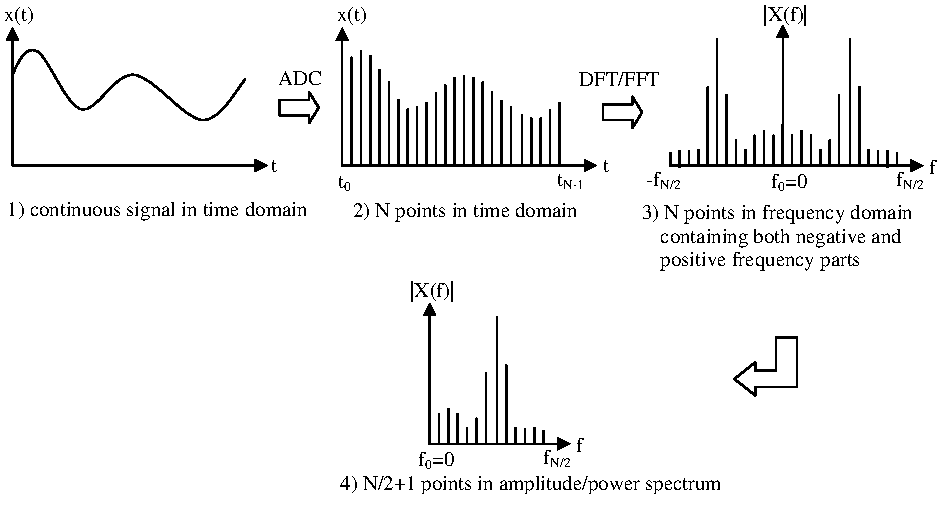
\includegraphics[width=\textwidth]{./img/fft1.pdf}
\end{figure}
\end{frame}
%-----------------------------------------------------------------------------

%-----------------------------------------------------------------------------
\begin{frame}{Fast Fourier Transform}
A transformada discreta de Fourier (DFT) de um vetor de $N$ pontos é:
\[
X_k = \sum_{n=0}^{N-1} x_n e^{-i 2 \pi k \frac{n}{N}}, \hspace{2em} k = 1, \dots, N-1.
\]
\begin{itemize}
  \item Implementação ingênua da DFT: $O(N^2)$.
  \item Implementações de FFT para diferentes valores de N: $O(N \log(N))$.
\end{itemize}
\end{frame}
%-----------------------------------------------------------------------------

%-----------------------------------------------------------------------------
\begin{frame}{Fast Fourier Transform}
\begin{figure}
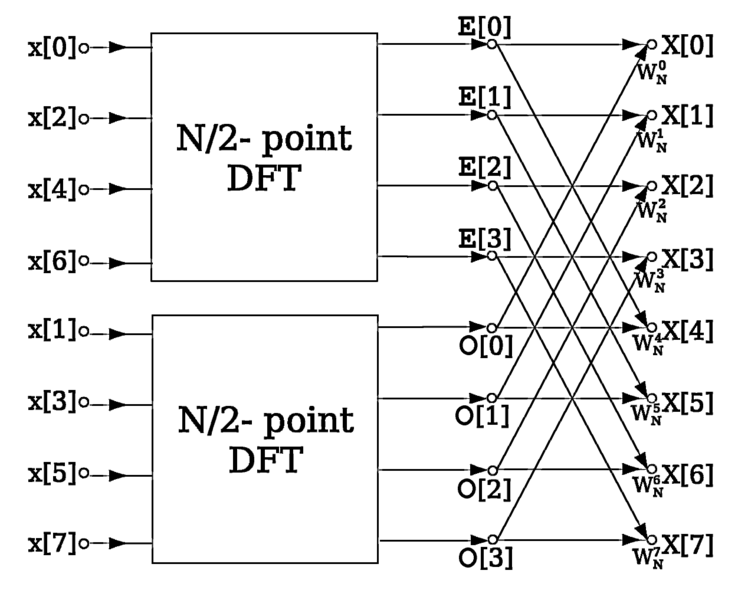
\includegraphics[height=0.8\textheight]{./img/butterfft.png}
\end{figure}
\end{frame}
%-----------------------------------------------------------------------------


%-----------------------------------------------------------------------------
%\begin{frame}{Fast Fourier Transform}
%Algoritmo de Cooley-Tukey para vetores de tamanho $2^k=2m$:
%\[
%  \begin{matrix} X_k & =
%& \sum \limits_{m=0}^{N/2-1} x_{2m}     e^{-\frac{2\pi i}{N} (2m)k}   +
%  \sum \limits_{m=0}^{N/2-1} x_{2m+1} e^{-\frac{2\pi i}{N} (2m+1)k}.
%  \end{matrix}
%\]
%Chamando de $E_k$ (e respectivamente $O_k$) o vetor de tamanho 2m com os
%índices pares (ímpares) $x_{2m}$ ($x_{2m+1}$), teremos:
%\[
%\begin{matrix} X_k & =
%& \left\{
%\begin{matrix}
%E_k + e^{-\frac{2\pi i}{N}k} O_k & \mbox{if } k < N/2 \\ \\
%E_{k-N/2} - e^{-\frac{2\pi i}{N} (k-N/2)} O_{k-N/2} & \mbox{if }
%k \geq N/2. \end{matrix} \right. \end{matrix}
%\]
%\end{frame}
%-----------------------------------------------------------------------------

%-----------------------------------------------------------------------------
\begin{frame}[fragile]{Fast Fourier Transform}
Código em altíssimo nível:
\begin{lstlisting}
four1(x, N, 1); /* O(N*log(N)) */
\end{lstlisting}
\begin{itemize}
  \item Qual é o tamanho máximo de uma FFT computável em tempo real?
\end{itemize}
\end{frame}
%-----------------------------------------------------------------------------


%-----------------------------------------------------------------------------
\begin{frame}{Fast Fourier Transform}{Resultados}
\begin{figure}
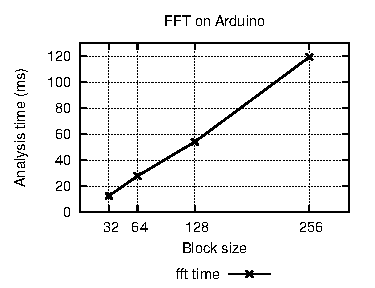
\includegraphics[width=0.8\textwidth]{./img/fft.pdf}
\end{figure}
\end{frame}
%-----------------------------------------------------------------------------

%-----------------------------------------------------------------------------
\begin{frame}{Fast Fourier Transform}{Resultados}
Determinação de frequência máxima:
\begin{itemize}
  \item Média de 428,15~$\mu$s por amostra.
  \item Frequência máxima $\approx$ 2.335~Hz.
  \item Pré-escalonador PWM de 32 $\Rightarrow$ $R=1.953$~Hz.
\end{itemize}
\end{frame}
%-----------------------------------------------------------------------------

%-----------------------------------------------------------------------------
\begin{frame}{Fast Fourier Transform}{Resultados}
\begin{figure}
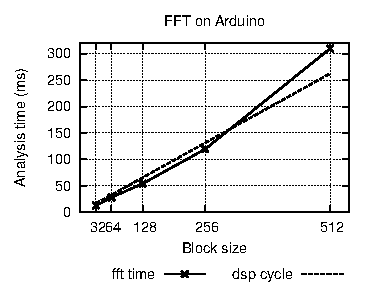
\includegraphics[width=0.8\textwidth]{./img/fft2.pdf}
\end{figure}
\end{frame}
%-----------------------------------------------------------------------------

